\chapter{Requirements}
%I dette afsnit beskrives krav til systemet med en kort beskrivelse af aktører, de vigtigste use-cases (funktionelle krav) og de vigtigste ikke-funktionelle krav. Beskrivelserne bør referere til kravspecifikationen i projektets bilag for yderligere detaljer. Ikke-funktionelle krav skal beskrives overordnet uden specifikke detaljer som f.eks. krav til værdier og nøjagtigheder, her henvises igen til kravspecifikationen i projektets bilag.

The Requirements for this project has been analyzed with the use of the MoSCoW method. This method is used to prioritize what should be worked on in the project. The method is separated into 4 levels of priority; \textbf{Must}, \textbf{Should}, \textbf{Could}, and \textbf{Won't}.

\noindent The following priorities have been chosen for this project:
\begin{itemize}
	\item[\textbf{Must}]
		\begin{itemize}
			\item Navigate waypoints from user input
			\item Be compatible with NMEA protocol GPS input
			\item Use GPS for localization
			\item Implement a PID control loop
		\end{itemize}
	\item[\textbf{Should}]
		\begin{itemize}
			\item Control thrusters in two-thruster catamaran
			\item Use a graphical user interface for user interaction
			\item Be able to change the PID parameters
		\end{itemize}
	\item[\textbf{Could}] 
		\begin{itemize}
			\item Control wheel in outboard motor on boat
			\item Be generic enough to use with other engine types
		\end{itemize}
	\item[\textbf{Won't}]
		\begin{itemize}
			\item Use pylogon-coverage for a specified area
			\item Avoid obstacles
		\end{itemize}
\end{itemize}

\section{Requirements specification}
To get a sense of the system, some mock-ups of a ui were created and can be found in the documentation in section~\ref{sec:mockups} on page~\pageref{sec:mockups}.

\begin{figure}[H]
\centering
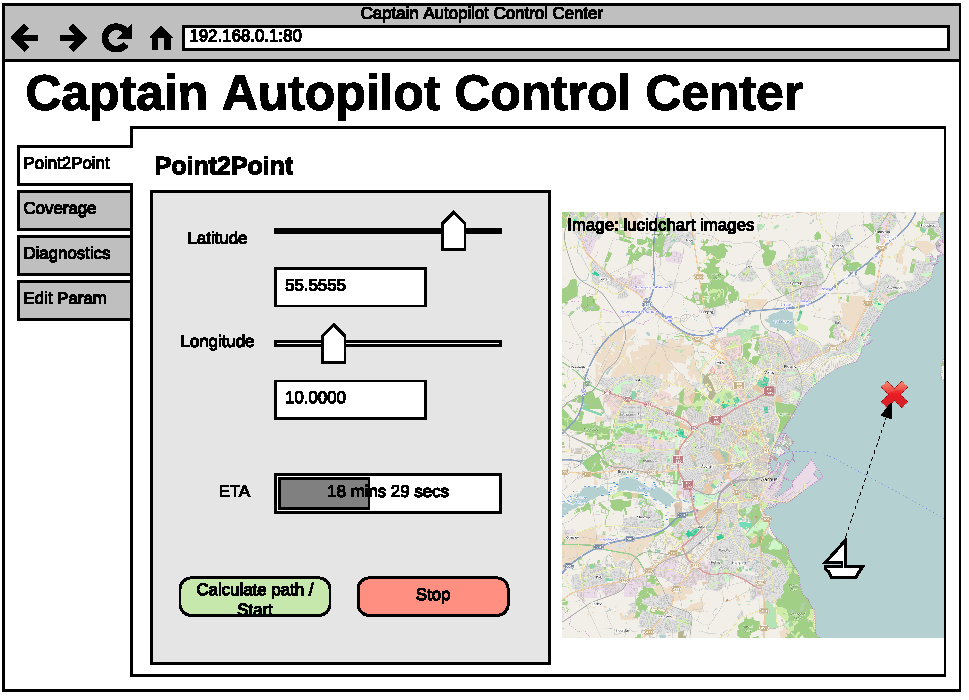
\includegraphics[width=0.7\linewidth]{../Appendix/Project/Dokumentation/Images/Requirements_specification/UI_Mockup_Point_to_point}
\caption{Mockup for the Point to point menu}
\label{fig:uimockuppointtopoint}
\end{figure}

An example of one of these mock ups is for describing a way point to navigate towards, can be seen in figure~\ref{fig:uimockuppointtopoint}. It describes how the a user should interact with the system, and how the system should communicate to the user.

To describe the functionallity in further detail, a user case driven approach has been used. First of all the actors of the system has to be identified. In figure~\ref{fig:uimockuppointtopoint} is the use case diagram for the system, on the right are the actors that initiate a use case. On the left the other actors are.

Initiating actors or primary actors of the CAPTAIN system, are a technician, and a user. The technician is an actor who setups the system, and has a more in depth knowledge of the system then the user. The user could be anyone, since all of the complicated work should be handled by the system or the technician. 

\begin{figure}[h]
\centering
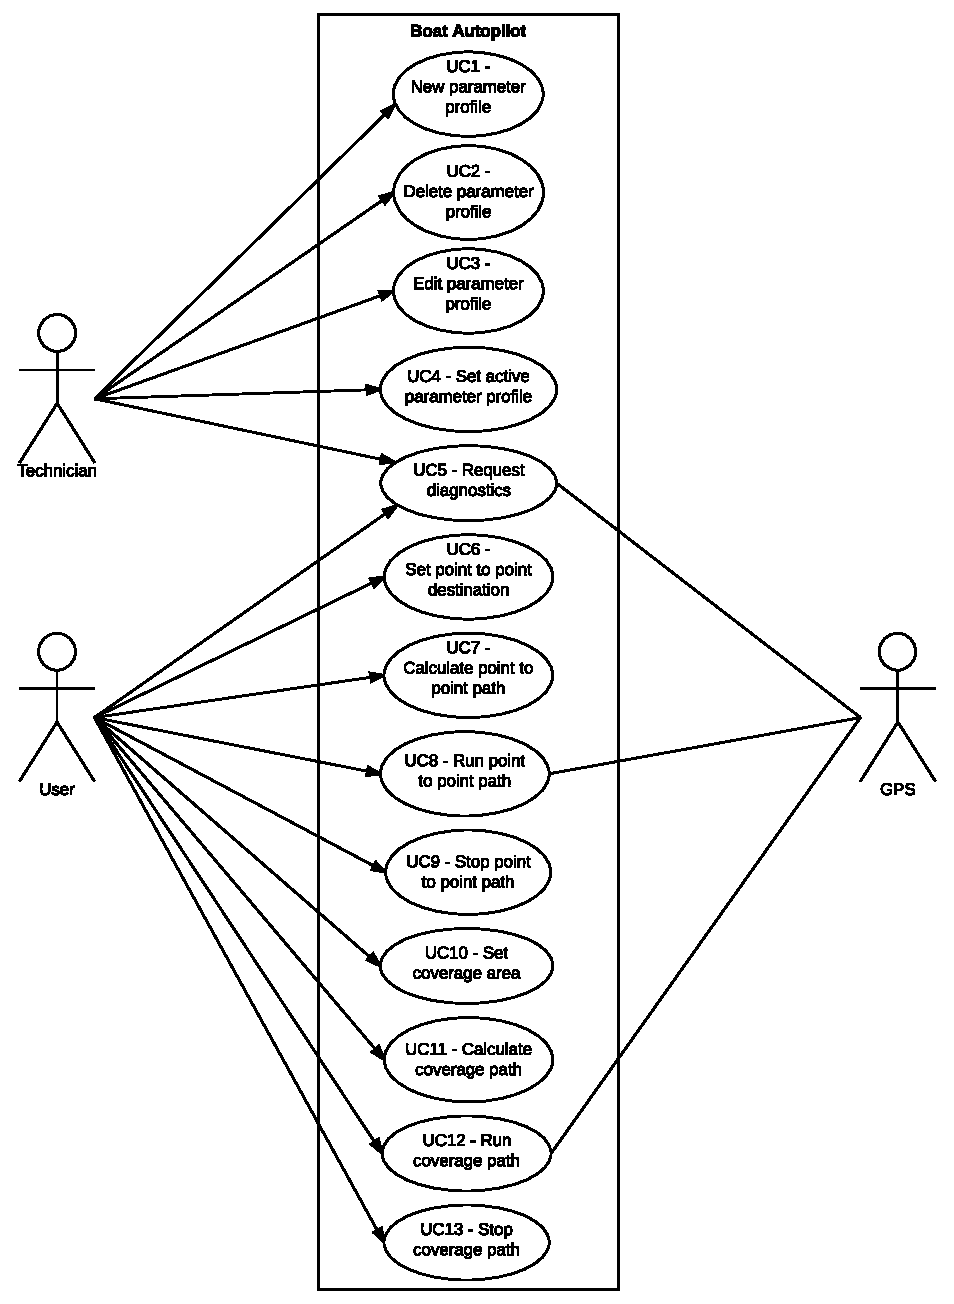
\includegraphics[width=0.7\linewidth]{../Appendix/Project/Dokumentation/Images/Requirements_specification/Usecase_diagram}
\caption{Use case diagram}
\label{fig:usecasediagram}
\end{figure}

The usecase diagram on figure~\ref{fig:usecasediagram} also list 13 different use cases. A use case describe a way to use the system, in this system they mainly describe a button of function that can be started by the user. In this section a few use cases will be looked at, but for all the fully dressed use cases, one can have a look at the documentation section ~\ref{sec:usecases} on page~\pageref{sec:usecases}.

\subsection{Use case 3 - Edit parameter profile}
One of the first things that was realized the system needed, was a way to describe parameters of the system. Parameters could be PID-loop terms, or the size of the boat, i fact anything that could be of use to the system. So to be able to save these parameters, the concepts of a parameter profile came to be. A parameters profile is essentially a list of any kind of parameters. Use case 3 - "Edit parameter profile", is the use case used to change the values of the of an already created parameter profile. It's important to note that it is the technician who initiates this use case, since know what exactly the values should be could require some deeper knowledge of the system. 

\subsection{Use case 11 - Calculate coverage path}
There are a tonne of ways to navigate way points, first of one needs to decide on how to describe a way points. So for this system way points can be describe in two ways, either as a single point, or as a rectangle. For the rectangle the system should calculate a path that covers a the rectangle with lines that have a predefined distance between them. This use case should be initialized by the user, as a simple press on the user interface. In return the user interface should display the calculated path, so the user can tell if the path is what they wanted.

\subsection{Use case 12 - Run coverage path}
With a calculated path, ei. list of way points to follow, the boat should be able to follow these points. When the user presses a button label "Run" Use case 12 - "Run coverage path" is initiated, and it should not finish until the boat has reached the last way point of the list of way points. The boat should get though the way points using a control loop. While the boat is running a the estimated time en-route should be displayed along with the current position of the boat.

\subsection{Use case 5 - Request diagnostics}
At any point in time, it might be convenient for the user or the technician, to know how the boat is doing. In other words, getting the diagnostics data from the boat. diagnostics data might include GPS information, what position the rudder is set to and so forth. This use case can, as mentioned be initiated by either the user or the technician, by the press of a button in the user interface. 



